\documentclass[aspectratio=169]{beamer}
\usetheme{Madrid}
\usecolortheme{default}
\usepackage{amsmath}
\usepackage{booktabs}
\usepackage{array}
\hypersetup{hidelinks}
\usepackage{xcolor}
\usepackage{tikz}
\usetikzlibrary{arrows.meta, positioning, shapes.geometric, calc}

% ---- GitHub hyperlink helpers (repo: BDeMo/research-notes) ----
\newcommand{\ghbase}{https://github.com/BDeMo/research-notes/blob/main/notes/plans/08-compressed-context-memory}
\newcommand{\ghB}[2]{\href{\ghbase/papers/paper-b-forgetting-gating/#1}{\color{blue}\underline{#2}}}
\newcommand{\ghC}[2]{\href{\ghbase/papers/paper-c-linear-attention/#1}{\color{blue}\underline{#2}}}
\newcommand{\best}[1]{\textbf{#1}}

\title[Long-Context Memory]{Long-Context Compression \& Linear-Attention Memory}
\subtitle{Research progress --- Papers A / B / C}
\author{Mingjia Shi}
\institute{RCA Foundation Model / Long-Context Memory}
\date{\today}

\begin{document}

\begin{frame}\titlepage
  \begin{center}\scriptsize All artifacts hyperlinked to
  \href{https://github.com/BDeMo/research-notes}{\color{blue}\underline{github.com/BDeMo/research-notes}} (blue = clickable).\end{center}
\end{frame}

% ============================ INDEX ============================
\begin{frame}{Outline / Index}
  \begin{columns}[T]
  \begin{column}{0.5\textwidth}
  \textbf{Part I --- Framing}
  \begin{enumerate}\small
    \item Background: the long-context memory wall
    \item One thesis, three papers (the mainline)
  \end{enumerate}
  \vspace{0.6em}
  \textbf{Part II --- Paper B (main result)}
  \begin{enumerate}\setcounter{enumi}{2}\small
    \item The diagnosis (model-invariant)
    \item The method: IMP router
    \item Full results table (all methods $\times$ benches)
    \item Honest standing vs \emph{all} baselines
    \item Rigor: a bug we found \& fixed
    \item Occam simplification $\to$ v3.0
  \end{enumerate}
  \end{column}
  \begin{column}{0.5\textwidth}
  \textbf{Part III --- Paper A (brief)}
  \begin{enumerate}\setcounter{enumi}{8}\small
    \item Learned soft-memory: honest negative
  \end{enumerate}
  \vspace{0.6em}
  \textbf{Part IV --- Paper C (next line)}
  \begin{enumerate}\setcounter{enumi}{9}\small
    \item Why linear attention; the research line
    \item The landscape (delta-rule family)
    \item GDN forgetting: exploration \& modules
  \end{enumerate}
  \vspace{0.6em}
  \textbf{Part V --- Wrap}
  \begin{enumerate}\setcounter{enumi}{12}\small
    \item Development logic \& timeline
    \item Cross-cutting insights \& next steps
    \item Artifact index (all links)
  \end{enumerate}
  \end{column}
  \end{columns}
\end{frame}

% ============================ PART I ============================
\section{Framing}
\begin{frame}{1. Background: the long-context memory wall}
  \textbf{Problem.} Softmax attention keeps a \emph{growing} KV cache: memory $\propto$ context length $L$.
  At 100k+ tokens this is the bottleneck for both cost and quality.
  \begin{itemize}
    \item \textbf{Two escape routes the field takes:}
    \begin{enumerate}
      \item \emph{Shrink the cache} --- KV-eviction (kvzip, knorm, SnapKV\ldots), prompt compression (LLMLingua), token merging (ToMe), retrieval (RAG).
      \item \emph{Remove the cache} --- \textbf{linear attention} / SSM (Mamba, RWKV, \textbf{Gated DeltaNet}): a \emph{fixed-size recurrent state}, $O(L)$ time, $O(1)$ memory.
    \end{enumerate}
    \item \textbf{Our base models} live in both worlds: Qwen3 (quadratic) and \textbf{Qwen3.5/3.6} (GDN linear-attention 3:1 hybrid).
  \end{itemize}
  \vspace{0.4em}
  \begin{block}{Guiding question}
  On a \emph{frozen} base, how do we feed / hold the \emph{right} context so long-context accuracy survives --- across architectures?
  \end{block}
\end{frame}

\begin{frame}{2. One thesis, three papers (the mainline)}
  \begin{block}{Thesis}
  Long-context accuracy is a \best{keep-the-answer-span} problem. No fixed compressor wins everywhere;
  the right mechanism is \best{input-adaptive} and, ideally, \best{training-free \& architecture-agnostic}.
  \end{block}
  \centering
  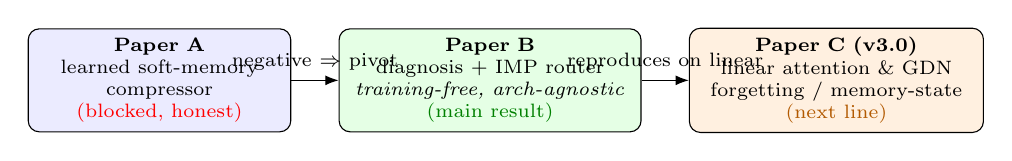
\begin{tikzpicture}[node distance=6mm, every node/.style={font=\scriptsize}]
    \node[draw,rounded corners,fill=blue!8,text width=3.1cm,align=center] (a) {\textbf{Paper A}\\learned soft-memory\\compressor\\\textcolor{red}{(blocked, honest)}};
    \node[draw,rounded corners,fill=green!10,text width=3.6cm,align=center,right=of a] (b) {\textbf{Paper B}\\diagnosis + IMP router\\\emph{training-free, arch-agnostic}\\\textcolor{green!50!black}{(main result)}};
    \node[draw,rounded corners,fill=orange!12,text width=3.5cm,align=center,right=of b] (c) {\textbf{Paper C (v3.0)}\\linear attention \& GDN\\forgetting / memory-state\\\textcolor{orange!70!black}{(next line)}};
    \draw[-{Latex}] (a) -- (b) node[midway,above]{negative $\Rightarrow$ pivot};
    \draw[-{Latex}] (b) -- (c) node[midway,above]{reproduces on linear};
  \end{tikzpicture}
  \vspace{0.4em}
  \footnotesize A learned compressor didn't beat commodity baselines (A) $\Rightarrow$ we shifted to \emph{diagnosing} what actually
  works and built a training-free router (B) $\Rightarrow$ the diagnosis holds on cache-free linear models, opening the linear-attention line (C).
\end{frame}

% ============================ PART II: Paper B ============================
\section{Paper B --- diagnosis + IMP}
\begin{frame}{3. Paper B --- the diagnosis (model-invariant)}
  Systematic full-test map across 9 model families (1.7B--14B, Qwen2.5/3/3.5, GLM-4, Ministral, Llama; quad + linear):
  \begin{itemize}
    \item \best{No universal compressor} --- the winner flips by task (retrieval / extractive / MC / reasoning).
    \item \best{``More context can hurt''} --- on literary-MC \emph{full} $<$ blind guessing (QuALITY full 7.2 $<$ 17.9); compression \emph{denoises}.
    \item \best{Retrieval $\gg$ full} on ultra-long ($\infty$Bench) --- selecting evidence beats reading everything.
    \item \best{Model-invariant}: the crossover \& denoising hold on \emph{every} family, incl. cache-free linear GDN.
  \end{itemize}
  \begin{block}{}
  \footnotesize This diagnosis --- not a single number --- is Paper B's durable contribution.
  \ghB{matrix-facts.md}{fact base (F27/F31/F43)} \; \ghB{main-table-fulltest.md}{full-test main table}
  \end{block}
\end{frame}

\begin{frame}{4. Paper B --- the method: IMP (Importance-routing Prefilter)}
  \textbf{Training-free, input-side, architecture-agnostic} prefilter on a \emph{frozen} base:
  \begin{enumerate}\small
    \item Score context tokens/chunks by cheap $O(L)$ signals (lexical BM25 + query-relevance + surprisal).
    \item Keep the top spans/chunks \emph{verbatim} to a budget; drop the rest. Feed to the frozen base.
    \item \best{Route} the granularity per input (\texttt{auto}): long/extractive $\to$ chunk-BM25 over the \emph{full doc}; literary-MC-that-fits $\to$ token-importance spans.
  \end{enumerate}
  \begin{itemize}\small
    \item No weights trained; runs on dense \emph{and} linear bases; no KV cache needed.
    \item Covers regimes that RAG (fails reasoning) and KV-eviction (can't run on linear) each only half-cover.
  \end{itemize}
  \begin{block}{}
  \footnotesize \ghB{method-vNext-2026-07-13.md}{method spec + code path} \; \ghB{imp-method-and-implementation.md}{implementation}
  \end{block}
\end{frame}

\begin{frame}{5. Paper B --- full results (Qwen3-8B, all methods $\times$ benches)}
  \centering\scriptsize
  \begin{tabular}{lccccccc}
  \toprule
  bench & full$\cdot$t & rag & kvzip$\ddagger$ & knorm$\ddagger$ & tome & \best{auto (ours)} & best \\
  \midrule
  $\infty$Bench (>100k) & 52.8 & 64.2 & 35.8 & 25.8 & 51.5 & \best{70.3} & \best{ours} \\
  RULER-NIAH & 99 & 94 & \best{99} & 85 & 0 & 98 & kvzip/ours* \\
  squad\_v2 & 65.9 & 67.2 & 64.9 & 16.5 & 38.9 & 66.9 & rag$\approx$ours \\
  trivia\_qa & 70.9 & 72.7 & 71.2 & 40.7 & 62.3 & \best{72.8} & \best{ours} \\
  lb\_multifieldqa & 38.6 & 38.8 & 37.1 & 30.7 & -- & \best{39.5} & \best{ours} \\
  lb\_narrativeqa & 14.0 & 13.7 & 11.2 & 9.3 & 13.5 & \best{14.3} & \best{ours} \\
  hotpot\_qa & 57.2 & 55.8 & 56.2 & 23.1 & 43.9 & 48.8 & full \\
  QuALITY-hard & 9.2 & 10.5 & \best{29.9} & 29.6 & 11.7 & 12.9 & \best{kvzip$\ddagger$} \\
  MuSR & 58.9 & 56.7 & 55.6 & 53.3 & 48.9 & 48.9 & full \\
  \bottomrule
  \end{tabular}
  \vspace{0.3em}
  \footnotesize $\cdot$t = truncated to 16k; $\ddagger$ = needs KV cache (\emph{cannot} run on linear). ours = \texttt{auto}.
  \ghB{COMPLETE-RESULTS-2026-07-13.md}{complete table (16 benches, 9 families)}
\end{frame}

\begin{frame}{6. Paper B --- honest standing vs \emph{all} baselines (not just RAG)}
  \begin{columns}[T]
  \begin{column}{0.52\textwidth}
  \textbf{Where ours wins / ties}
  \begin{itemize}\small
    \item \best{Wins}: $\infty$Bench, trivia, multifieldqa, narrativeqa.
    \item \best{Ties best}: squad, lb\_hotpotqa, ms\_marco, LongBench-v2; best \emph{arch-agnostic} on RULER.
    \item \best{Only method that runs on linear} among the strong ones.
  \end{itemize}
  \end{column}
  \begin{column}{0.48\textwidth}
  \textbf{Where we honestly lose}
  \begin{itemize}\small
    \item \textcolor{red}{Literary-MC} (QuALITY) $\to$ \emph{KV-eviction} (kvzip/knorm $\approx$30) --- but they need a KV cache.
    \item \textcolor{red}{Dense reasoning} (MuSR, musique) $\to$ \emph{full} (needs everything).
  \end{itemize}
  \end{column}
  \end{columns}
  \vspace{0.4em}
  \begin{block}{Framing for the paper}
  \footnotesize Contribution = the \best{diagnosis} + a \best{regime-spanning training-free router}, \emph{not} ``beats everything''.
  We state plainly where KV-eviction / full win. \ghB{best-of-all-baselines-2026-07-13.md}{best-of-all comparison}
  \end{block}
\end{frame}

\begin{frame}{7. Paper B --- rigor: a bug we found \& fixed}
  \begin{itemize}
    \item \textbf{Symptom:} IMP looked $-19$ vs RAG on $\infty$Bench.
    \item \textbf{Root cause (case-level audit):} IMP \emph{truncated} the context to 16k \emph{before} selecting; RAG retrieved over the \emph{whole} 131k-token doc. \best{87\% of RAG's kept content came from beyond 16k --- IMP was structurally blind to it.}
    \item \textbf{Fix:} chunk-family retrieves over the full doc (no forward needed). $\infty$Bench $51 \to \best{76}$ --- the gap \emph{reversed} to a win.
    \item \textbf{Discipline installed:} every result labels \texttt{full$\cdot$trunc16k}; per-bench truncated-vs-true-full audited; only $\infty$Bench materially affected.
  \end{itemize}
  \begin{block}{}
  \footnotesize \ghB{correctness-audit-2026-07-13.md}{correctness audit} \; \ghB{imp-vs-rag-case-diff-2026-07-13.md}{case-level diff} \; \ghB{code-review-2026-07-13.md}{code review}
  \end{block}
\end{frame}

\begin{frame}{8. Paper B --- Occam simplification $\to$ v3.0}
  \textbf{What actually drives the wins?} An ablation of the (baroque) \texttt{auto} router shows:
  \begin{itemize}\small
    \item The \best{chunk branch = full-doc BM25 retrieval} carries nearly all the wins.
    \item Importance signals (surprisal, query-dot) add $\approx 0$; the span branch only matters in literary-MC (where it still loses to KV-eviction).
  \end{itemize}
  \begin{block}{v3.0 = \texttt{IMP-lite}: one mode, one signal, one knob}
  \footnotesize Full-document lexical chunk retrieval on a frozen base --- no span mode, no surprisal, no router, no training.
  Occam: drop every non-load-bearing part; keep the workhorse. \ghB{method-vNext-2026-07-13.md}{v3.0 design + validation plan}
  \end{block}
  \footnotesize \emph{Open question (decide empirically):} is IMP-lite meaningfully $>$ RAG, or is it ``RAG configured for compression + the diagnosis''?
\end{frame}

% ============================ PART III: Paper A ============================
\section{Paper A}
\begin{frame}{9. Paper A --- learned soft-memory: an honest negative}
  \begin{itemize}
    \item \textbf{Idea:} compress context into a few learned \emph{soft tokens} on a frozen base (+ a do-no-harm gate).
    \item \textbf{Findings (honest):}
    \begin{itemize}\small
      \item The compressor is a \best{commodity} --- flipping any single loss moves accuracy $\pm0.03$.
      \item Learned soft-memory \best{cannot compress extractive QA} (squad $\approx$ no-context); \emph{training-free IMP beats it on the same task}.
      \item The reconstruction-based gate was a \best{non-effect} (AUROC $\approx$ chance).
    \end{itemize}
    \item \textbf{Outcome:} Paper A's learned compressor is the blocker $\Rightarrow$ this \emph{motivated} the pivot to Paper B's training-free direction.
  \end{itemize}
  \begin{block}{}\footnotesize \ghB{PAPER-A-v1.8.1-complete.md}{Paper A spec} \; \ghB{negative-results.md}{negative results}\end{block}
\end{frame}

% ============================ PART IV: Paper C ============================
\section{Paper C --- linear attention}
\begin{frame}{10. Paper C (v3.0) --- why linear attention; the research line}
  \textbf{Focus (next line):} linear attention \& its variants (Qwen3.5/3.6 GDN family; \emph{no} Qwen3 control).
  \begin{itemize}\small
    \item \textbf{The tension:} a \emph{fixed-size state} is efficient but has a structural \best{recall / forgetting bottleneck} (recall--throughput tradeoff; state-tracking limits).
    \item \textbf{Our hook (already shown):} on Qwen3.5-GDN the long-context diagnosis reproduces, but \best{KV-eviction can't even run} (no KV) --- only input-side selection (IMP-lite/RAG) works.
    \item \textbf{The opening:} on linear bases the problem isn't ``shrink the KV'' (there is none) --- it's \best{feed the right small context / augment the state's recall}.
  \end{itemize}
  \begin{block}{Candidate spine}
  \footnotesize C-1 diagnose GDN forgetting (no training) + C-2 training-free input-side memory (IMP-lite) that KV-methods structurally can't provide. \ghC{PAPER-C-research-line.md}{research line}
  \end{block}
\end{frame}

\begin{frame}{11. Paper C --- the landscape (delta-rule family)}
  \centering\scriptsize
  \begin{tabular}{lcccc}
  \toprule
  model & decay & erase & write & delta \\
  \midrule
  Mamba-2 & scalar & --- & scalar & no \\
  \textbf{Gated DeltaNet} (our base) & scalar & tied scalar & tied scalar & yes \\
  KDA / Kimi-Linear & channel-wise & tied scalar & tied scalar & yes \\
  \textbf{GDN-2} (NVIDIA, 2026) & channel-wise & \best{channel-wise} & \best{channel-wise} & yes \\
  \bottomrule
  \end{tabular}
  \vspace{0.5em}
  \begin{itemize}\footnotesize
    \item Frontier = \best{how to \emph{edit} the compressed memory} (erase vs write) without scrambling associations.
    \item Field findings: the \emph{delta rule} dominates recall; \best{GDN-2's erase gate carries most of its gain} (selective forgetting of stale keys is the lever); channel-wise helps long-range but can hurt precise recall.
  \end{itemize}
  \begin{block}{}\footnotesize \ghC{references-linear-attention.md}{reference collection (11 categories, arXiv)}\end{block}
\end{frame}

\begin{frame}{12. Paper C --- GDN forgetting: exploration \& modules}
  \textbf{Training-free anti-forgetting modules tested on Qwen3.5-GDN (real benches):}
  \centering\scriptsize
  \begin{tabular}{lccccc}
  \toprule
  bench & full & imp-lite & rel-last & replay & rag \\
  \midrule
  $\infty$Bench & 55 & 76 & 75 & \best{78} & 65 \\
  lb\_multifieldqa & 38.6 & 42.1 & 40.7 & \best{44.0} & 41.1 \\
  babilong-qa1 & 65 & \best{68} & 62 & 61 & 54 \\
  \bottomrule
  \end{tabular}
  \vspace{0.4em}
  \begin{itemize}\footnotesize
    \item \best{Input-side compression rescues GDN on ultra-long} ($\infty$Bench 55$\to$76) --- don't overflow the fixed state.
    \item Recency-reorder modules (rel-last / replay) = \emph{marginal, task-dependent} $\Rightarrow$ Occam: imp-lite default.
    \item \textcolor{red}{Honesty:} our synthetic single-needle probe was \emph{inconclusive} (task too easy / a probe bug we caught); the trustworthy evidence is the \emph{real-bench} grid above. 128k probe OOMs (GDN kernel).
  \end{itemize}
  \begin{block}{}\footnotesize \ghC{gdn-forgetting-exploration.md}{ablation design} \; \ghC{gdn-module-results-2026-07-14.md}{module results (+ probe caveats)}\end{block}
\end{frame}

% ============================ PART V: Wrap ============================
\section{Wrap}
\begin{frame}{13. Development logic \& timeline}
  \begin{enumerate}\small
    \item \textbf{Paper A} --- learned soft-memory compressor $\to$ honest negatives (commodity compressor, gate a non-effect).
    \item \textbf{Pivot} --- stop building a compressor; \emph{diagnose} what works on a frozen base.
    \item \textbf{Paper B} --- full-test diagnosis (model-invariant) + IMP router; iterated token$\to$span$\to$+lexical$\to$5-mode$\to$\texttt{auto}$\to$full-doc.
    \item \textbf{Rigor pass} --- case-level audit found the truncation bug (F44), fixed it, re-ran the corrected main table, best-of-all-baselines, code review.
    \item \textbf{Occam} --- ablate to \texttt{IMP-lite} (v3.0); own the honest scope.
    \item \textbf{Paper C} --- the diagnosis reproduces on linear GDN where KV-methods can't run $\to$ new line on linear-attention forgetting.
  \end{enumerate}
\end{frame}

\begin{frame}{14. Cross-cutting insights \& next steps}
  \textbf{Insights}
  \begin{itemize}\small
    \item Long-context = \best{keep-the-gold-span}; \emph{gold-recall predicts accuracy}.
    \item \best{No universal compressor}; the right granularity is \emph{input-dependent}; retrieval can \emph{denoise above full}.
    \item Diagnosis is \best{model-invariant}; KV-eviction owns literary-MC but \best{can't run on linear} --- that gap is ours.
  \end{itemize}
  \textbf{Next steps}
  \begin{itemize}\small
    \item \textbf{Paper B:} run the IMP-lite Occam ablation; finalize v3.0; decide the RAG-delta claim.
    \item \textbf{Paper C:} secure the in-band \best{Qwen3.6-27B} (hybrid) checkpoint; RULER access (HF); diagnose GDN forgetting on real long-context; test input-side vs erase-gate-retrofit fixes.
  \end{itemize}
\end{frame}

\begin{frame}{15. Artifact index (all links to GitHub)}
  \scriptsize
  \textbf{Paper B} \quad
  \ghB{REPORT-2026-07-13.md}{consolidated report} $\cdot$
  \ghB{COMPLETE-RESULTS-2026-07-13.md}{complete results} $\cdot$
  \ghB{main-table-fulltest.md}{main table} $\cdot$
  \ghB{matrix-facts.md}{fact base} $\cdot$
  \ghB{best-of-all-baselines-2026-07-13.md}{best-of-all} \\
  \ghB{correctness-audit-2026-07-13.md}{correctness audit} $\cdot$
  \ghB{code-review-2026-07-13.md}{code review} $\cdot$
  \ghB{method-vNext-2026-07-13.md}{v3.0 method} $\cdot$
  \ghB{FIVE-DAY-SUMMARY-2026-07-08_13.md}{5-day summary}
  \vspace{0.7em}

  \textbf{Paper A} \quad \ghB{PAPER-A-v1.8.1-complete.md}{spec} $\cdot$ \ghB{negative-results.md}{negatives}
  \vspace{0.7em}

  \textbf{Paper C} \quad
  \ghC{README.md}{overview} $\cdot$
  \ghC{PAPER-C-research-line.md}{research line} $\cdot$
  \ghC{references-linear-attention.md}{references} $\cdot$
  \ghC{gdn-forgetting-exploration.md}{GDN forgetting design} $\cdot$
  \ghC{gdn-module-results-2026-07-14.md}{module results}
  \vspace{0.9em}

  \centering \normalsize Repo: \href{https://github.com/BDeMo/research-notes}{\color{blue}\underline{github.com/BDeMo/research-notes}}
\end{frame}

\end{document}
